%package list
\documentclass{article}
\usepackage[top=3cm, bottom=3cm, outer=3cm, inner=3cm]{geometry}
\usepackage{multicol}
\usepackage{graphicx}
\usepackage{url}
%\usepackage{cite}
\usepackage{hyperref}
\usepackage{array}
%\usepackage{multicol}
\newcolumntype{x}[1]{>{\centering\arraybackslash\hspace{0pt}}p{#1}}
\usepackage{natbib}
\usepackage{pdfpages}
\usepackage{multirow}
\usepackage[normalem]{ulem}
\useunder{\uline}{\ul}{}
\usepackage{svg}
\usepackage{xcolor}
\usepackage{listings}
\lstdefinestyle{ascii-tree}{
	literate={├}{|}1 {─}{--}1 {└}{+}1 
}
\lstset{basicstyle=\ttfamily,
	showstringspaces=false,
	commentstyle=\color{red},
	keywordstyle=\color{blue}
}
%\usepackage{booktabs}
\usepackage{caption}
\usepackage{subcaption}
\usepackage{float}
\usepackage{array}
\usepackage{enumitem}
\usepackage[utf8]{inputenc}
\newcolumntype{M}[1]{>{\centering\arraybackslash}m{#1}}
\newcolumntype{N}{@{}m{0pt}@{}}


%%%%%%%%%%%%%%%%%%%%%%%%%%%%%%%%%%%%%%%%%%%%%%%%%%%%%%%%%%%%%%%%%%%%%%%%%%%%
%%%%%%%%%%%%%%%%%%%%%%%%%%%%%%%%%%%%%%%%%%%%%%%%%%%%%%%%%%%%%%%%%%%%%%%%%%%%
\newcommand{\itemEmail}{sdiazt@unsa.edu.pe}
\newcommand{\itemStudent}{Sebastian Diaz Ticona}
\newcommand{\itemCourse}{Programación Web 2}
\newcommand{\itemSemester}{III}
\newcommand{\itemUniversity}{Universidad Nacional de San Agustín de Arequipa}
\newcommand{\itemFaculty}{Facultad de Ingeniería de Producción y Servicios}
\newcommand{\itemDepartment}{Departamento Académico de Ingeniería de Sistemas e Informática}
\newcommand{\itemSchool}{Escuela Profesional de Ingeniería de Sistemas}
\newcommand{\itemAcademic}{2023 - A}
\newcommand{\itemInput}{Del 22 Abril 2023}
\newcommand{\itemOutput}{Al 07 Junio 2023}
\newcommand{\itemPracticeNumber}{04}
\newcommand{\itemTheme}{Python}
%%%%%%%%%%%%%%%%%%%%%%%%%%%%%%%%%%%%%%%%%%%%%%%%%%%%%%%%%%%%%%%%%%%%%%%%%%%%
%%%%%%%%%%%%%%%%%%%%%%%%%%%%%%%%%%%%%%%%%%%%%%%%%%%%%%%%%%%%%%%%%%%%%%%%%%%%

\usepackage[english,spanish]{babel}
\AtBeginDocument{\selectlanguage{spanish}}
\renewcommand{\figurename}{Figura}
\renewcommand{\refname}{Referencias}
\renewcommand{\tablename}{Tabla} %esto no funciona cuando se usa babel
\AtBeginDocument{%
	\renewcommand\tablename{Tabla}
}

\usepackage{fancyhdr}
\pagestyle{fancy}
\fancyhf{}
\setlength{\headheight}{30pt}
\renewcommand{\headrulewidth}{1pt}
\renewcommand{\footrulewidth}{1pt}
\fancyhead[L]{\raisebox{-0.2\height}{
\includegraphics[width=3cm]{img/logo_episunsa.png}}}
\fancyhead[C]{\fontsize{7}{7}\selectfont	\itemUniversity \\ \itemFaculty \\ \itemDepartment \\ \itemSchool \\ \textbf{\itemCourse}}
\fancyhead[R]{\raisebox{-0.2\height}{
\includegraphics[width=1.2cm]{img/logo_abet}}}
\fancyfoot[L]{Estudiante: Sebastian Diaz Ticona}
\fancyfoot[C]{\itemCourse}
\fancyfoot[R]{Página \thepage}

% para el codigo fuente
\usepackage{listings}
\usepackage{color, colortbl}
\definecolor{dkgreen}{rgb}{0,0.6,0}
\definecolor{gray}{rgb}{0.5,0.5,0.5}
\definecolor{mauve}{rgb}{0.58,0,0.82}
\definecolor{codebackground}{rgb}{0.95, 0.95, 0.92}
\definecolor{tablebackground}{rgb}{0.8, 0, 0}



\lstset{frame=tb,
	language=bash,
	aboveskip=3mm,
	belowskip=3mm,
	showstringspaces=false,
	columns=flexible,
	basicstyle={\small\ttfamily},
	numbers=none,
	numberstyle=\tiny\color{gray},
	keywordstyle=\color{blue},
	commentstyle=\color{dkgreen},
	stringstyle=\color{mauve},
	breaklines=true,
	breakatwhitespace=true,
	tabsize=3,
	backgroundcolor= \color{codebackground},
}

\usepackage{selinput}
\SelectInputMappings{
	aacute={á},
	ntilde={ñ},
	Euro={€}
}

\begin{document}
	
	\vspace*{10px}
	
	\begin{center}	
		\fontsize{17}{17} \textbf{ Informe de Laboratorio \itemPracticeNumber}
	\end{center}
	\centerline{\textbf{\Large Tema: \itemTheme}}		
	
	\begin{table}[H]
		\begin{tabular}{|x{4.7cm}|x{4.8cm}|x{4.8cm}|}
			\hline 
			\rowcolor{tablebackground}
			\color{white} \textbf{Estudiante} & \color{white}\textbf{Escuela}  & \color{white}\textbf{Asignatura}   \\
			\hline 
			{\itemStudent \par \itemEmail} & \itemSchool & {\itemCourse \par Semestre: \itemSemester }     \\
			\hline 			
		\end{tabular}
	\end{table}	
	
	\begin{table}[H]
		\begin{tabular}{|x{4.7cm}|x{4.8cm}|x{4.8cm}|}
			\hline 
			\rowcolor{tablebackground}
			\color{white}\textbf{Laboratorio} & \color{white}\textbf{Tema}  & \color{white}\textbf{Duración}   \\
			\hline 
			\itemPracticeNumber & \itemTheme & 04 horas   \\
			\hline 
		\end{tabular}
	\end{table}
	
	\begin{table}[H]
		\begin{tabular}{|x{4.7cm}|x{4.8cm}|x{4.8cm}|}
			\hline 
			\rowcolor{tablebackground}
			\color{white}\textbf{Semestre académico} & \color{white}\textbf{Fecha de inicio}  & \color{white}\textbf{Fecha de entrega}   \\
			\hline 
			\itemAcademic & \itemInput &  \itemOutput  \\
			\hline 
		\end{tabular}
	\end{table}
	
	\section{Tarea}
	\begin{itemize}		
		\item Para resolver los siguientes ejercicios solo está permitido usar ciclos, condicionales, definición de listas por comprensión, sublistas, \texttt{map}, \texttt{join}, \texttt{(+)}, \texttt{lambda}, \texttt{zip}, \texttt{append}, \texttt{pop}, \texttt{range}.
		\begin{itemize}[leftmargin=2em]
			\item[a)] Implemente los métodos de la clase \texttt{Picture}. Se recomienda que implemente la clase \texttt{Picture} por etapas, probando realizar los dibujos que se muestran en la siguiente pregunta.
		\end{itemize}
		\begin{itemize}[leftmargin=2em]
			\item[b)] Usando únicamente los métodos de los objetos de la clase \texttt{Picture}, dibuje las siguientes figuras (invoque a \texttt{draw}):
			\\
			
			\subitem(a)
			\begin{figure}[ht]
				\centering
				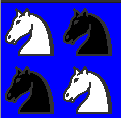
\includegraphics[scale=2.7]{img/ejercicio_02_a}
				\caption{}
			\end{figure}
			
			
			\subitem(b)
			\begin{figure}[ht]
				\centering
				
\includegraphics[scale=2.7]{img/ejercicio_02_b}
				\caption{}
			\end{figure}
			
			\newpage
			\subitem(c)
			\begin{figure}[ht]
				\centering
				
\includegraphics[scale=3.5]{img/ejercicio_02_c}
				\caption{}
			\end{figure}
			
			
			\subitem(d)
			\begin{figure}[ht]
				\centering
				
\includegraphics[scale=2.5]{img/ejercicio_02_d}
				\caption{}
			\end{figure}
			
			\subitem(e)
			\begin{figure}[ht]
				\centering
				
\includegraphics[scale=2.5]{img/ejercicio_02_e}
				\caption{}
			\end{figure}
			
			\subitem(f)
			
			
			\begin{minipage}{\linewidth}
				\centering
				
\includegraphics[scale=2.9]{img/ejercicio_02_f}
				\captionof{figure}{}
			\end{minipage}
			
			\newpage
			\subitem(g)
			\begin{figure}[ht]
				\centering
				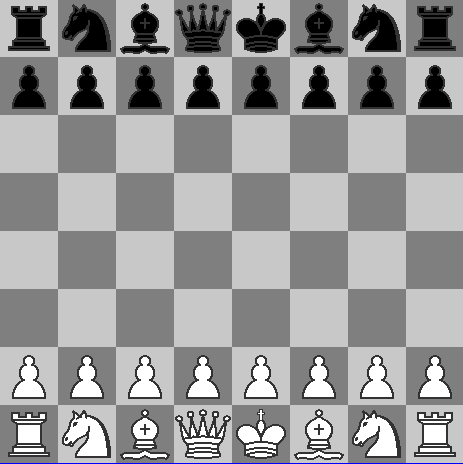
\includegraphics[scale=2.5]{img/ejercicio_02_g}
				\caption{}
			\end{figure}
			
			
		\end{itemize}
	\end{itemize}
	
	\section{Equipos, materiales y temas utilizados}
	\begin{itemize}
		\item Sistema Operativo Windows 10.
		\item VIM 9.0.
		\item Python 3.11.3.
		\item Pip 23.1.2
		\item Pygame 2.4.0
		\item Git 2.41.0.
		\item Cuenta en GitHub con el correo institucional.
		\item Programación Orientada a Objetos.	
	\end{itemize}
	
	\section{URL de Repositorio Github}
	\begin{itemize}
		\item URL del Repositorio GitHub.
		\item \url{https://github.com/Sebastian04081/Lab04-Pweb2.git}
		\item URL para el laboratorio 04 en el Repositorio GitHub.
		\item \url{https://github.com/rescobedoq/pw2/tree/main/labs/lab04}
	\end{itemize}
	
	
	
	\section{Actividades con el repositorio GitHub}
	
	\subsection{Creando e inicializando repositorio GitHub}
	\begin{itemize}	
		\item Se creo el repositorio GitHub.
		\item Se realizaron los siguientes comandos en la computadora:
	\end{itemize}	
	
	\begin{lstlisting}[language=bash,caption={Creando directorio de trabajo}][H]
		$ mkdir ~/workspace/Pweb2/
	\end{lstlisting}
	\begin{lstlisting}[language=bash,caption={Dirijíéndonos al directorio de trabajo}][H]
		$ cd ~/workspace/Pweb2/
	\end{lstlisting}	
	\begin{lstlisting}[language=bash,caption={Creando directorio para repositorio GitHub}][H]
		$ mkdir Lab04-Pweb2/
	\end{lstlisting}
	\begin{lstlisting}[language=bash,caption={Inicializando directorio para repositorio GitHub}][H]
		$ git init
		$ git remote add origin https://github.com/Sebastian04081/Lab04-Pweb2.git
	\end{lstlisting}
	
	\begin{lstlisting}[language=bash,caption={Inicializando directorio para crear el entorno virtual}][H]
		$ pip install virtualenv
		$ mkdir ./my_env
		$ source my_env/Scripts/activate
	\end{lstlisting}
	
	\begin{lstlisting}[language=bash,caption={Instalando pygame para poder trabajar los ejercicios propuestos}][H]
		$ pip install pygame
		$ pip list
		Package    Version
		---------- -------
		pip        23.1.2
		pygame     2.4.0
		setuptools 67.7.2
		wheel      0.40.0
	\end{lstlisting}
	
	\begin{lstlisting}[language=bash,caption={Inicializando directorio para cargar los archivos .py}][H]
		$ mkdir ./src
		$ cd ./src
		$ ls -l
		total 52
		drwxr-xr-x 1 __pycache__/
		-rw-r--r-- 1 chessPictures.py
		-rw-r--r-- 1 colors.py
		-rw-r--r-- 1 Ejercicio2a.py
		-rw-r--r-- 1 Ejercicio2b.py
		-rw-r--r-- 1 Ejercicio2c.py
		-rw-r--r-- 1 Ejercicio2d.py
		-rw-r--r-- 1 Ejercicio2e.py
		-rw-r--r-- 1 Ejercicio2f.py
		-rw-r--r-- 1 Ejercicio2g.py
		-rw-r--r-- 1 interpreter.py
		-rw-r--r-- 1 picture.py
		-rw-r--r-- 1 pieces.py
	\end{lstlisting}
	
	\subsection{Commits}
	\begin{lstlisting}[language=bash,caption={Primer Commit Creando carpeta/src para los archivos .py}][H]
		$ git add .
		$ git commit -m "Agregando los archivos .py"			
		$ git push -u origin main
	\end{lstlisting}
	
	\begin{itemize}	
		\item Se creo el archivo \textbf{.gitignore} para no considerar los archivos \textbf{*.class} que son innecesarios hacer seguimiento.
	\end{itemize}
	\begin{lstlisting}[language=bash,caption={Creando requirements.txt}][H]
		$ vim ../requirements.txt
	\end{lstlisting}
	\begin{lstlisting}[language=bash,caption={../requirements.txt}][H]
		pygame==2.4.0
	\end{lstlisting}
	\begin{lstlisting}[language=bash,caption={Commit: Creando requirements.txt para especificar las verciones de las librerias}][H]
		$ git add .
		$ git commit -m "Agregando el archivo requirements.txt"			
		$ git push -u origin main
	\end{lstlisting}
	
	\begin{itemize}	
		\item Para el siguiente commit se implemento los métodos de la clase picture.py.
		\item Los métodos implementados son los siguientes:
	\end{itemize}	
	
	\lstinputlisting[language=Python, caption={picture.py},numbers=left,]{../src/picture.py}
	
	\begin{lstlisting}[language=bash,caption={Para el siguiente commit se implementaron los Ejercicios 2a hasta el 2g.}][H]
		$ ls -l
		total 56
		drwxr-xr-x 1 __pycache__/
		-rw-r--r-- 1 chessPictures.py
		-rw-r--r-- 1 colors.py
		-rw-r--r-- 1 Ejercicio2a.py
		-rw-r--r-- 1 Ejercicio2b.py
		-rw-r--r-- 1 Ejercicio2c.py
		-rw-r--r-- 1 Ejercicio2d.py
		-rw-r--r-- 1 Ejercicio2e.py
		-rw-r--r-- 1 Ejercicio2f.py
		-rw-r--r-- 1 Ejercicio2g.py
		-rw-r--r-- 1 interpreter.py
		-rw-r--r-- 1 picture.log
		-rw-r--r-- 1 picture.py
		-rw-r--r-- 1 pieces.py
	\end{lstlisting}
		
	
	\lstinputlisting[language=Python, caption={Ejercicio2a.py},numbers=left,]{../src/Ejercicio2a.py}
	
	\lstinputlisting[language=Python, caption={Ejercicio2b.py},numbers=left,]{../src/Ejercicio2b.py}
	
	\lstinputlisting[language=Python, caption={Ejercicio2c.py},numbers=left,]{../src/Ejercicio2c.py}
	
	\lstinputlisting[language=Python, caption={Ejercicio2d.py},numbers=left,]{../src/Ejercicio2d.py}
	
	\lstinputlisting[language=Python, caption={Ejercicio2e.py},numbers=left,]{../src/Ejercicio2e.py}
	
	\lstinputlisting[language=Python, caption={Ejercicio2f.py},numbers=left,]{../src/Ejercicio2f.py}
	
	\lstinputlisting[language=Python, caption={Ejercicio2g.py},numbers=left,]{../src/Ejercicio2g.py}
	
	
	\subsection{Estructura de laboratorio 04}
	\begin{itemize}	
		\item El contenido que se entrega en este laboratorio es el siguiente:
	\end{itemize}
	
	\begin{lstlisting}[style=ascii-tree]
		Lab04-Pweb2/
		|--- requirements.txt
		|--- Informe
		|    |--- Informe_Lab04(Python).pdf
		|    |--- img
		|	       |--- logo_abet.png
		| 	       |--- logo_episunsa.png
		| 	       |--- logo_unsa.jpg
		| 	       |--- ejercicio_02_a.png
		| 	       |--- ejercicio_02_b.png
		| 	       |--- ejercicio_02_c.png
		| 	       |--- ejercicio_02_d.png
		| 	       |--- ejercicio_02_e.png
		| 	       |--- ejercicio_02_f.png
		| 	       |--- ejercicio_02_g.png
		|
		|--- src
		|    |--- chessPictures.py
		|    |--- colors.py
		|    |--- Ejercicio2a.py
		|    |--- Ejercicio2b.py
		|    |--- Ejercicio2c.py
		|    |--- Ejercicio2d.py
		|    |--- Ejercicio2e.py
		|    |--- Ejercicio2f.py
		|    |--- Ejercicio2g.py
		|    |--- interpreter.py
		|    |--- picture.log
		|    |--- picture.py
		|    |--- pieces.py
	\end{lstlisting}
	
	\section{Cuestionario}
	\begin{itemize}
		\item ¿Qué son los archivos *.pyc? \\ \\
		Los archivos '.pyc' son archivos de código de byte compilado en Python. Cuando se ejecuta un archivo de Python, el intérprete de Python compila el código fuente en un formato de código de byte que es más eficiente para la ejecución. Estos archivos '.pyc' contienen el código de byte compilado y se utilizan para acelerar la carga y ejecución de un módulo o programa en Python.
		\item ¿Para qué sirve el directorio pycache? \\ \\
		El directorio '\_\_pycache\_\_', a menudo denominado 'pycache', es utilizado por el intérprete de Python para almacenar los archivos .pyc. Es un directorio especial creado automáticamente cuando se compila un archivo .py y se almacenan allí los archivos .pyc correspondientes. El propósito principal de este directorio es mantener los archivos compilados en un lugar separado para evitar la necesidad de recompilarlos cada vez que se ejecute el programa.
		\item ¿Cuáles son los usos y lo que representa el subguión en Python? \\ \\
		El subguión (\_) en Python se utiliza para indicar que un elemento no es relevante en un contexto específico. También se usa en importaciones especiales y para marcar cadenas de texto que deben ser traducidas en aplicaciones internacionales.
	\end{itemize}	
	
	\section{Referencias}
	\begin{itemize}			
		\item \url{https://www.w3schools.com/python/python_reference.asp}
		\item \url{https://docs.python.org/}
		\item \url{https://www.geeksforgeeks.org/python-programming-language/}
	\end{itemize}	

\end{document}